\documentclass{szzclass}

\usepackage{amsmath}
\usepackage{graphics}
% \usepackage[czech]{babel}
% \usepackage[margin=3cm]{geometry}
% \usepackage{wrapfig}

% spacing
\usepackage{titlesec}
% \titlespacing*{\section}{0pt}{1ex}{0.5ex}
\titlespacing*{\subsection}{0pt}{1ex}{0ex}

% \topic{Binární haldy, binomiální haldy. Vyhledávací stromy a   jejich vyvažování. Tabulky s rozptylováním (hešováním).}
\title{Binární haldy, binomiální haldy. Vyhledávací stromy a   jejich vyvažování. Tabulky s rozptylováním (hešováním).}
\renewcommand*\contentsname{Obsah}
\author{Daniel Hampl}
% \code{BI-SPOL-5}
% \subject{AG1}

\begin{document}
\maketitle

\tableofcontents
\newpage

\section{Binární haldy}

\begin{figure}[h]
\centering
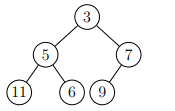
\includegraphics[width=0.4\textwidth]{topics/bi-spol-5/images/binary-heap.png}
\end{figure}

Binární minimová halda je datová struktura tvaru binárního
stromu, v jehož každém vrcholu $x$ je uložen jeden klíč $k(x)$, a která
splňuje tyto dvě vlastnosti:
\begin{itemize}
    \item \textbf{Tvar haldy}: Strom má všechny hladiny kromě poslední plně
    obsazené. Poslední hladina je zaplněna od levého okraje směrem k pravému.
    \item \textbf{Haldové uspořádání}: Je-li $v$ vrchol a $s$ jeho syn, plat $k(v) ≤ k(s)$.
    \item Binární halda s $n$ prvky má $\lfloor $log $ n \rfloor + 1$ hladin.
    \item Binární halda s $n$ prvky má $\lceil n/2\rceil$ listů a $\lfloor n/2 \rfloor$ vnitřních vrcholů.
\end{itemize}

\subsection{Vložení prvku do haldy}
\begin{itemize}
    \item $O($log$~n)$
    \item Tvar haldy dovoluje přidat okamžitě nový prvek na konec nejspodnější hladiny.
    \item Pokud by již byla plná, založíme novou hladinu.
    \item Pokud je haldové uspořádání mezi novým listem $l$ a jeho otcem $o$ v pořádku, můžeme skončit. Pokud ne, prohodíme $k(l)$ a $k(o)$.
    \item Tím ale může nastat problém mezi klíčem vrcholu $o$ a klíčem otce vrcholu $o$ $\implies$  prohodíme a opakujeme BubbleUp
\end{itemize}

\subsection{Odstranění minima}
\begin{itemize}
    \item $O($log$~n)$
    \item Odstranění kořene r stromu haldy by porušilo vlastnost Tvar haldy.
    \item Prohoď klíče vrcholů $root$ a $last$, odstraň vrchol $last$ a potom přesuň klíč z $root$ na správné místo tak, aby opět platilo haldové uspořádání. BubbleDown
\end{itemize}

\subsection{Reprezentace pomocí pole}
Kořen haldy uložíme do nultého prvku pole ($array[0]$). Poté pro každý prvek $array[n]$ jsou jeho následníci uloženi v $array[2n+1]$ a $array[2n+2]$.


\section{Binominální strom}

\begin{figure}[h]
\centering
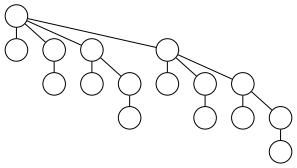
\includegraphics[width=0.4\textwidth]{topics/bi-spol-5/images/binominal-tree.png}
\end{figure}

Binomiální strom řádu $k$ (značíme $B_k$) je uspořádaný (záleží na
pořadí synů) zakořeněný strom, pro který platí:
\begin{itemize}
    \item $B_0$ je tvořen pouze kořenem.
    \item Pro $k \geq 1$ získáme $B_k$ ze stromů $B_0, B_1, . . . , B_k−1$ tak, že
    přidáme nový kořen a kořeny těchto stromů uděláme (takto
    popořadě) syny nového kořene.
\end{itemize}

\begin{figure}[h!]
\centering
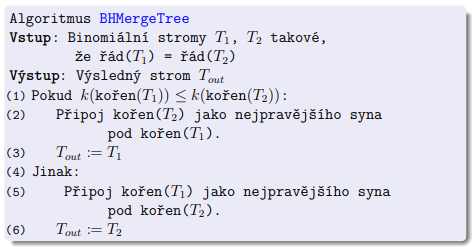
\includegraphics[width=0.8\textwidth]{topics/bi-spol-5/images/BHMerge.png}
\end{figure}

\newpage

\section{Binominální halda}

\begin{figure}[h]
\centering
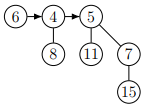
\includegraphics[width=0.4\textwidth]{topics/bi-spol-5/images/binominal-heap.png}
\end{figure}

Binomiální halda obsahující $n$ prvků se skládá ze souboru
binomiálních stromů $T = T_1, . . . , T_i$, kde
\begin{itemize}
    \item Uchovávané prvky jsou uloženy ve vrcholech stromů $T_i$.
    Prvek uložený ve vrcholu $v \in V(T_i)$ značíme $k(v)$.
    \item  Pro každý strom $T_i$ platí tzv. haldové uspořádání, neboli pro
    každý $v \in V(T_i)$ a jeho syny $s_1, . . . , s_k$ platí $k(v) \leq k(s_j)$,
    $j = 1, . . . , k$.
    \item V souboru $T$ se žádný řád binomiálního stromu nevyskytuje
    dva- nebo vícekrát.
    \item Soubor stromů $T$ je uspořádán vzestupně podle jejich řádů
    (tedy podle stupňů jejich kořenů a tedy podle velikosti).
\end{itemize}

Binomiální strom $B_k$ se vyskytuje v souboru stromů $n$-prvkové
binomiální haldy právě tehdy, když je v dvojkovém zápisu čísla $n$
nastavený $k$-tý nejnižší bit na 1.

$n$-prvková binomiální halda sestává z $O($log $n)$ binomiálních stromů.


\textbf{Složitost}
\begin{itemize}
    \item Vložení $O($log $n)$
    \item Nalezení minima $O(1)$
    \item Extrakce minima $O($log $n)$
    \item Merge $O($log $n)$
    \item Build $O(n)$
    \item Delete $O($log $n)$
\end{itemize}


\textbf{Merge} hald probíhá stejně, jako sčítání dvou binárních číísel.


\newpage

\section{Vyhledávací stromy}

\subsection{BVS}

\begin{figure}[h]
\centering
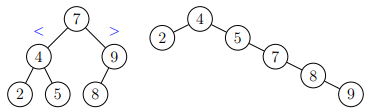
\includegraphics[width=0.4\textwidth]{topics/bi-spol-5/images/bvs.png}
\end{figure}

Binární vyhledávací strom (BVS) je binární strom, v jehož
každému vrcholu $v$ je uložen unikátní klíč $k(v)$. Přitom pro každý
vrchol $v$ musí platit:
\begin{itemize}
    \item Pokud $a \in L(v)$, pak $k(a) < k(v)$ .
    \item Pokud $b \in R(v)$, pak $k(b) > k(v)$.
\end{itemize}

Binární vyhledávací strom nazveme dokonale vyvážený, pokud pro každý jeho vrchol v platí $|L(v)|~-~|R(v)|~\leq~1$.

\textbf{Složitost} základních operací na BVS je průměrně $O($log $n)$, ale může dosáhnout až $O(n)$.

\subsection{AVL}

Binární vyhledávací strom nazveme AVL stromem, pokud pro každý
jeho vrchol v platí $h(l(v)) − h(r(v)) \leq 1$.

Budeme v každém vrcholu $v$ udržovat číslo $δ(v) = h(r(v)) - h(l(v))$, které nazveme znaménko vrcholu $v$.

V korektním AVL stromu může nabývat jen těchto hodnot:
\begin{itemize}
    \item δ(v) = +1 (pravý podstrom hlubší) – takový vrchol značíme \textcircled{$+$},
    \item δ(v) = −1 (levý podstrom hlubší) – značíme \textcircled{$-$},
    \item δ(v) = 0 (oba podstromy stejně hluboké) – značíme \textcircled{$\cdot$}.
\end{itemize}

\textbf{Složitost} základních operací na AVL je $O($log $n)$.

% \begin{figure}[h]
% \centering
% 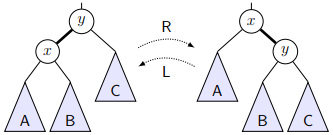
\includegraphics[width=0.4\textwidth]{topics/bi-spol-5/images/avl1.PNG}
% \end{figure}

% \begin{figure}[h]
% \centering
% 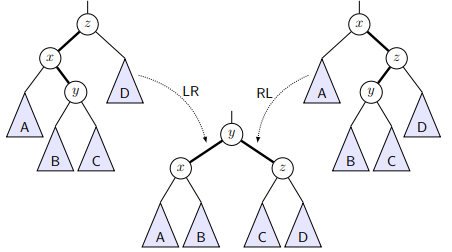
\includegraphics[width=0.6\textwidth]{topics/bi-spol-5/images/avl2.PNG}
% \end{figure}

\begin{figure}[!h]
	\centering
	\begin{minipage}{0.39\textwidth}
		\centering
        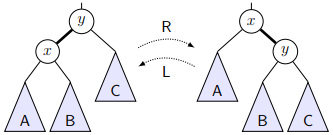
\includegraphics[width=\textwidth]{topics/bi-spol-5/images/avl1.png}
	\end{minipage}
	\begin{minipage}{0.59\textwidth}
		\centering
        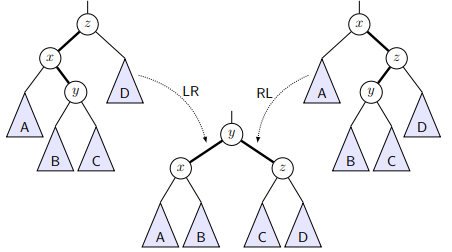
\includegraphics[width=\textwidth]{topics/bi-spol-5/images/avl2.png}
	\end{minipage}
\end{figure}

\newpage


\section{Hešovací tabulky}

\subsection{Hašování s řetízky}
Prvky jsou ukládány do pole či spojového seznamu odpovídající příslušnmu haši.

\begin{figure}[h!]
\centering
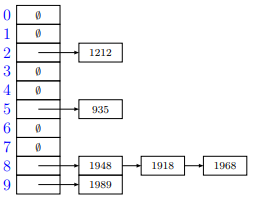
\includegraphics[width=0.5\textwidth]{topics/bi-spol-5/images/hashRetizky.png}
\end{figure}

\subsection{Otevřená adresace}
Prvky jsou ukládány na další ásledující místo v poli získané za pomoci dvojité hašovací funkce. V přpadě mazání prvku se zamění za značku smazaného prvku, který značí možnou existenci dalších prvků s ekvivalentním hašem. 
Následně, pokud narazíme na značku smazaného prvku při vkládání, tak se prvek vloží na míísto značky. V případě, že na tuto znařku narazíme při vyhledávání, tak pokračujeme na další iteraci algoritmu, jako kdyby zde byl platný prvek.


\textbf{Dvojité hešování}:\newline Prohledávací posloupnost je dána funkcí
$h(k, i) = (f(k) + i \cdot g(k)) \text{mod } m$, kde $f : U \rightarrow \{0, . . . , m - 1\}$ a
$g : U → \{1, . . . , m - 1\}$ jsou dvě různé hešovací funkce, $m$ je
prvočíslo a $i$ je počet neúspěšných pokusů v aktuální operaci
Protože je $m$ prvočíslo, je s ním $g(k)$ vždy nesoudělné a
posloupnost navštíví každou přihrádku právě jednou.

\begin{figure}[h!]
\centering
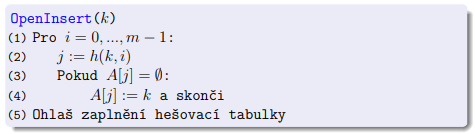
\includegraphics[width=0.8\textwidth]{topics/bi-spol-5/images/hashOpenInsert.png}
\end{figure}

\end{document}